\documentclass[12pt]{article}


\newcommand{\GroupId}{idk}
\newcommand{\assignment}{project-security}

\NeedsTeXFormat{LaTeX2e}
\usepackage[osf]{mathpazo}
\usepackage[svgnames]{xcolor}
\usepackage[T1]{fontenc}
\usepackage{amsmath,amsthm,amsfonts,amssymb,mathtools}
\usepackage{hyperref,url}
\usepackage{float}
\usepackage[margin=2.7cm,a4paper]{geometry}
\usepackage{tasks}
\usepackage{xstring}
\usepackage[tikz]{mdframed}
\usepackage{environ}
\usepackage{subcaption}
\usepackage{etoolbox}
\usepackage{fourier-orns}
\usepackage{kvoptions}
\usepackage[]{units}
\usepackage{url}%
%\usepackage[normal]{subfigure}

% math config

\DeclarePairedDelimiter\ceil{\lceil}{\rceil}
\DeclarePairedDelimiter\abs{\lvert}{\rvert}
\DeclarePairedDelimiter\set{\{}{\}}


% headers

\usepackage{fancyhdr}
\addtolength{\headheight}{2.5pt}
\pagestyle{fancy}
\fancyhead{} 
\fancyhead[L]{\sc info2222} % Replace with comp2123 or comp2823
\renewcommand{\headrulewidth}{0.75pt}

% update these headers
\fancyhead[C]{\sc Group Id: \GroupId}
\fancyhead[R]{Assignment \assignment}

\begin{document}

\section{Introduction}

This assignment is actually much better than Comp2017's o.O

\section{Approach explanation}
    \subsection*{Part: Basic Functionality Requirements:}
        \subsubsection*{1} Basically provided by template...

        \subsubsection*{2} Once user logs in successfully, a dynamic friend list can be shown bottom right the webpage. It displays all the users who this user is friend with as buttons. By clicking on the bottoms, the user can join in the chat room and chat with the friend. In order to implement this feature, we designed a class called friendship (shown in Figure \ref{friendshipClass}) , then we use a function called get friends for user, to get all the users who this user if friend with.(shown in Figure \ref{getfriends}) . Then we use a function called fetchfriends in the frontend to display all the friends as buttons. Once clicking the bottom, it will trigger join room function, which allows user to chat with friends(shown in Figure \ref{fetchfriends}).

        \subsubsection*{3} The user can send a friend request to the other user by entering the username(shown in Figure \ref{enterusername}). We designed a class called FriendRequest to implement this feature (shown in Figure \ref{friendrequestClass}). Once entering the username, the server will check whether the username exists. If the username is valid, then it will check whether they are already been friends\ref{sendfriendrequest}. If so, the friend request will not be sent.
	
	   \subsubsection*{4} Once the user trying to send a friend request, if the users are already friends, the request will not be send and will not be displayed. Otherwise, the request will be displayed dynamically to both sender and receiver. The sender will see a message which shows "To: receiver", while the receiver will see "From: sender", with two buttons "Accept" and "Reject"(shown in Figure \ref{twobuttons}) . Once the receiver accept the friendship request, the status will be updated \ref{updatestatus} , and the receiver will become a friend of the sender and will be shown in the friend list immediately. Otherwise if the receiver reject the request, the status will also be updated immediately and this request will disappear automatically.  In order to achieve the dynamic part, we applyed socket to listen to the friendrequest(shown in Figure  \ref{fetchrequests} Figure \ref{requestsocketio}) , so it will update the friend requests automatically without manual refresh.
        \newpage

        \subsubsection*{5} 

        All the friends of the user is displayed as buttons in the friend list (shown in Figure \ref{friendlist}).  Once clicking on the button, it will call the join room function which allows the user to join in their friend's chat room.  To ensure that both user and friend are currently online so they can communicate securely, we add a get users in room medthod for the room class, which checks whether both of them are in the room.(shown in Figure \ref{getusersinroom}). Then we use this method when trying to send messages (shown in Figure \ref{send}).   

        \textbf{The process of ensuring secure communication between users:}
        \begin{enumerate}
            \item When a user successfully logs in or signs up, they generate a pair of cryptographic keys: a public key and a private key as shown in Figure \ref{show_keys}.

            As shown in Figure \ref{generate_key_pairs}, the process begins with hashing the password using the SHA-256 hash function to create a fixed-length seed. This enhances security by mitigating risks associated with using raw passwords and provides necessary entropy. The SHA-256 hash output, initially an ArrayBuffer, is then converted into a Uint8Array, and finally into a hexadecimal string to format the seed for key generation. Using this processed seed, the ec.genKeyPair function from the elliptic library is utilized to generate the ECC key pair, as demonstrated in the cryptographic process.

            Subsequently, the frontend stores both the public key and the private key as shown in \ref{store_key_pairs}. The public key is uploaded to the server using an axios request and stored in a database called public\_keys, as shown in Figures \ref{Upload and Store public key} and \ref{db public_key}. Meanwhile, the private key is retained in the user's local storage, as shown in Figure \ref{local_storage}.. These keys are generated based on the user's password, ensuring that they are consistently the same each time they are generated.

		\begin{figure}[H]
                \centering
                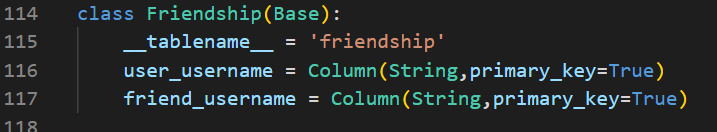
\includegraphics[width=0.8\textwidth]{zzrgraphs/models_friendship.png}
                \caption{models.py define a class called friendship}
                \label{friendshipClass}
            \end{figure}

		\begin{figure}[H]
                \centering
                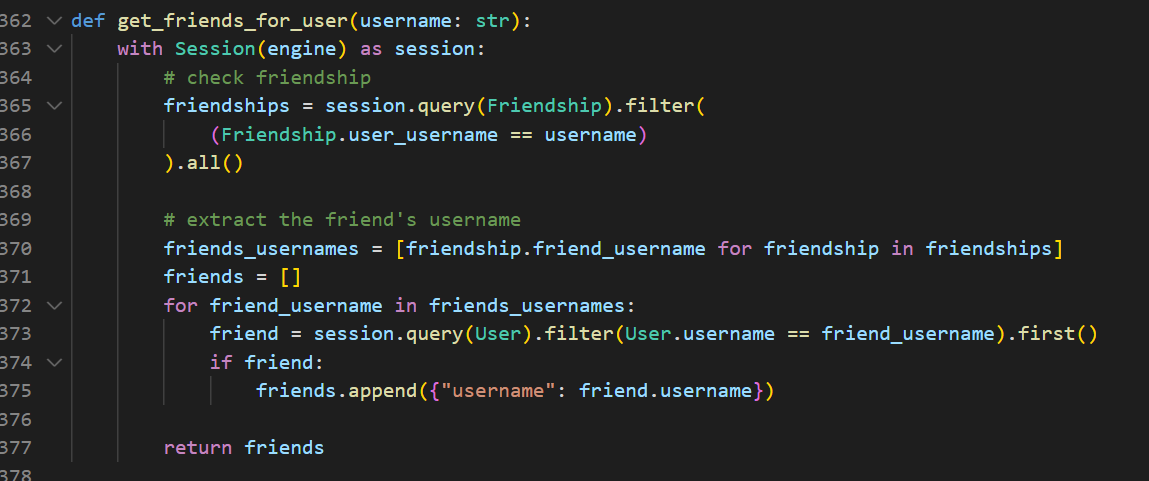
\includegraphics[width=0.8\textwidth]{zzrgraphs/db_getfriendforuser.png}
                \caption{db.py get all the friends of the current user}
                \label{getfriends}
            \end{figure}

		\begin{figure}[H]
                \centering
                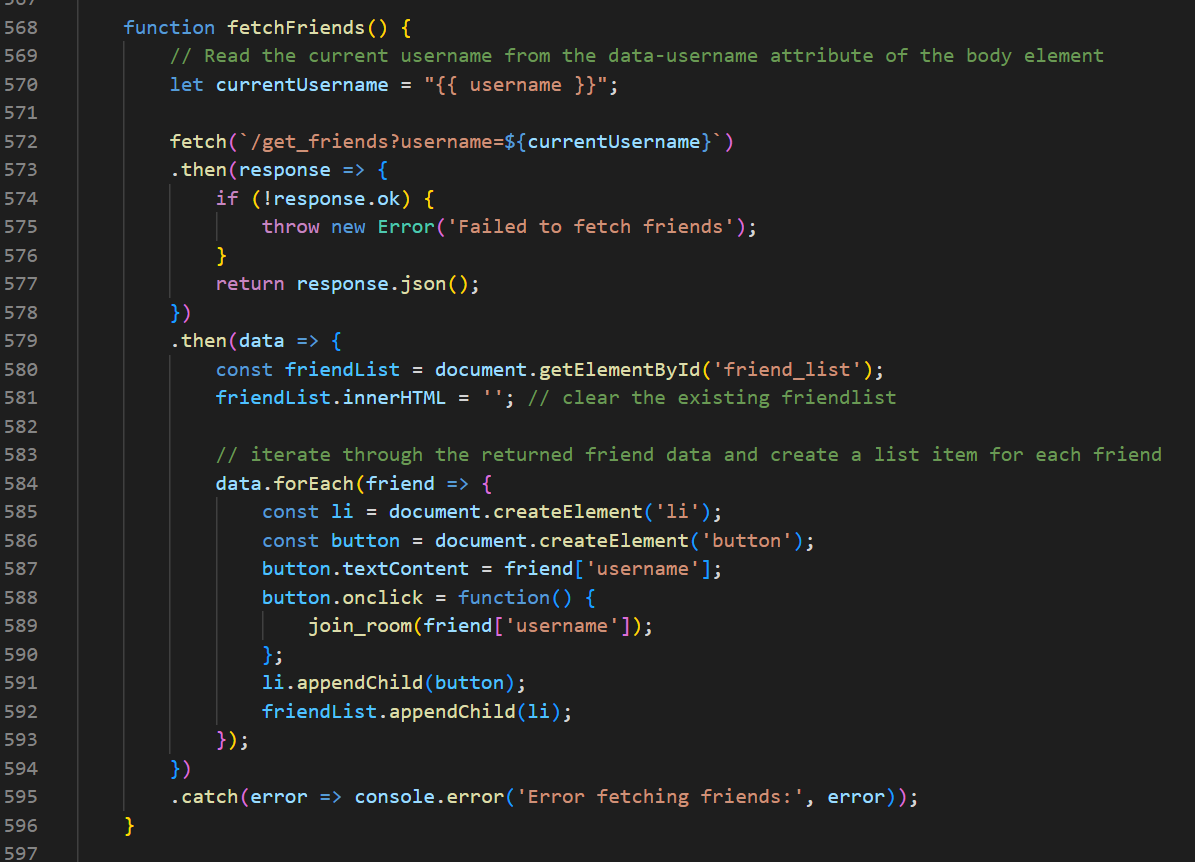
\includegraphics[width=0.8\textwidth]{zzrgraphs/home_fetchFriends.png}
                \caption{home.jinja fetch friends function}
                \label{fetchfriends}
            \end{figure}

		\begin{figure}[H]
                \centering
                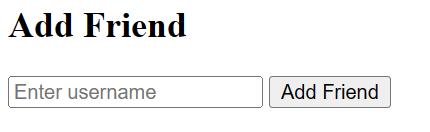
\includegraphics[width=0.4\textwidth]{zzrgraphs/enter_username.png}
                \caption{home page: add friend feature}
                \label{enterusername}
            \end{figure}

		\begin{figure}[H]
                \centering
                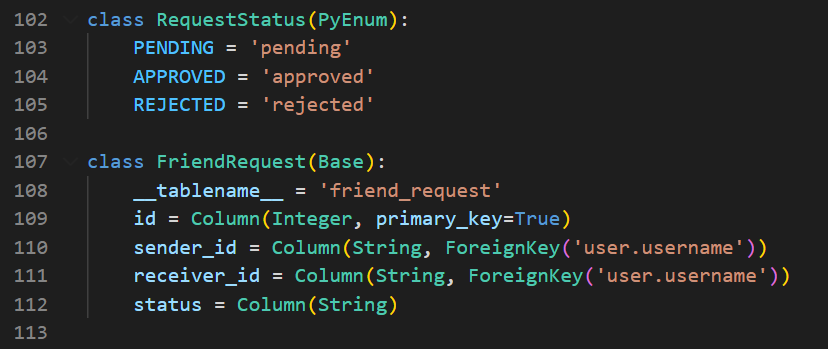
\includegraphics[width=0.8\textwidth]{zzrgraphs/models_friendrequest.png}
                \caption{models.py define a class called friendrequest}
                \label{friendrequestClass}
            \end{figure}

		\begin{figure}[H]
                \centering
                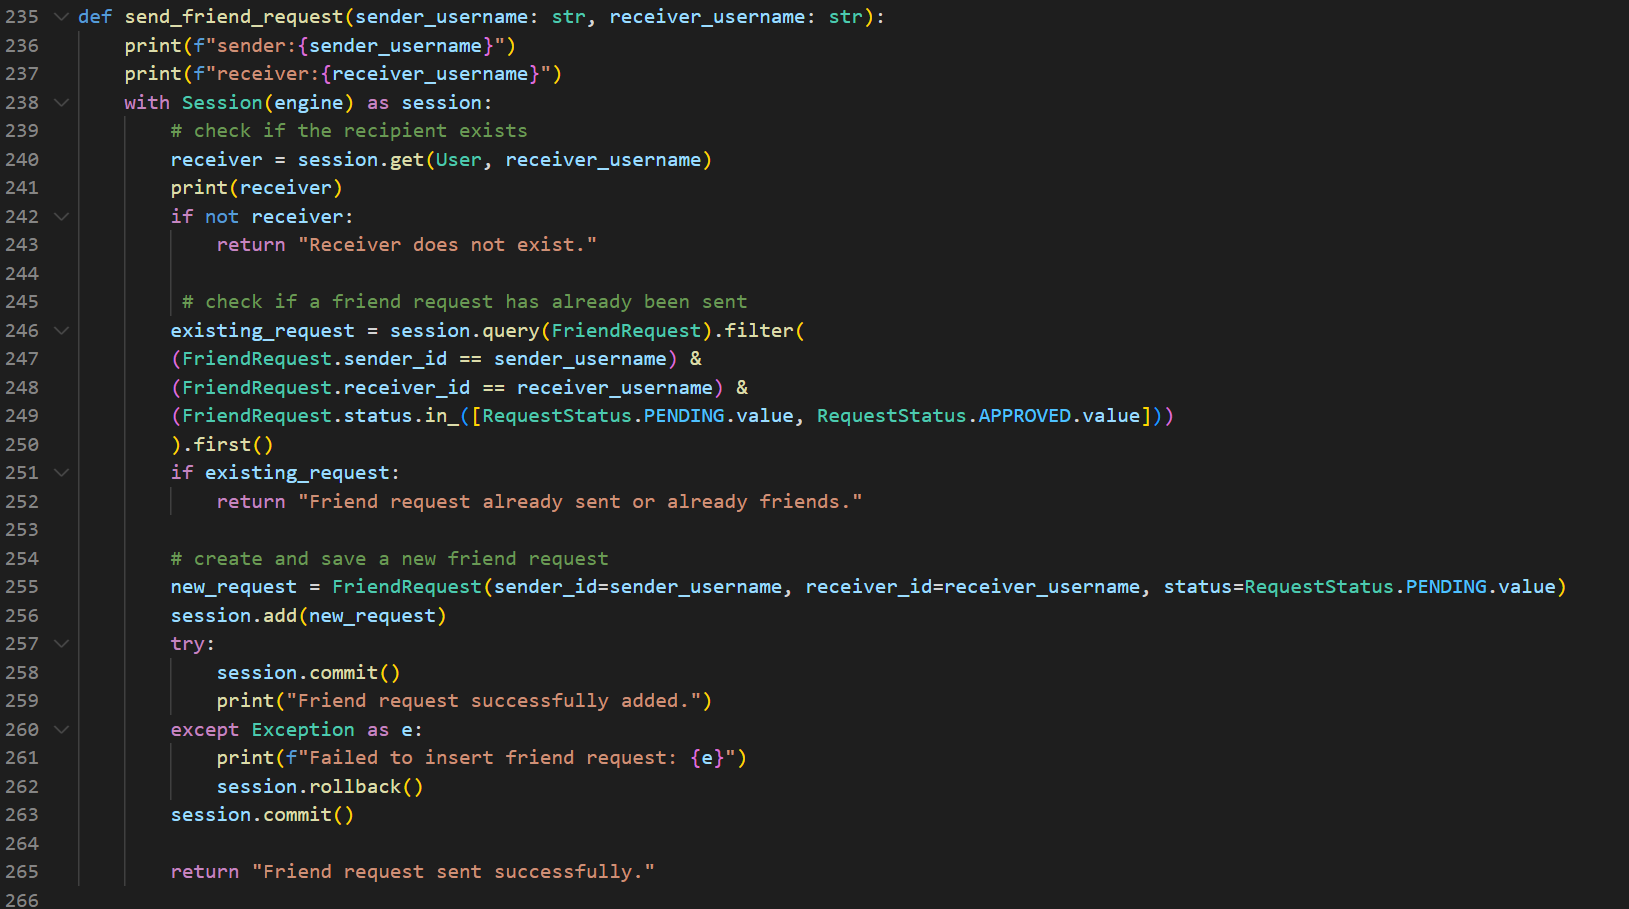
\includegraphics[width=0.8\textwidth]{zzrgraphs/db_send_friend_request.png}
                \caption{db.py send friend request to the other user}
                \label{sendfriendrequest}
            \end{figure}

		\begin{figure}[H]
                \centering
                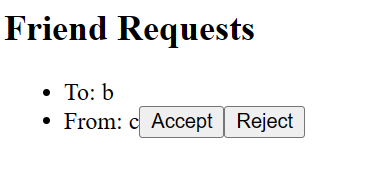
\includegraphics[width=0.4\textwidth]{zzrgraphs/display_friendrequests.png}
                \caption{home page: display friend requests}
                \label{twobuttons}
            \end{figure}

		\begin{figure}[H]
                \centering
                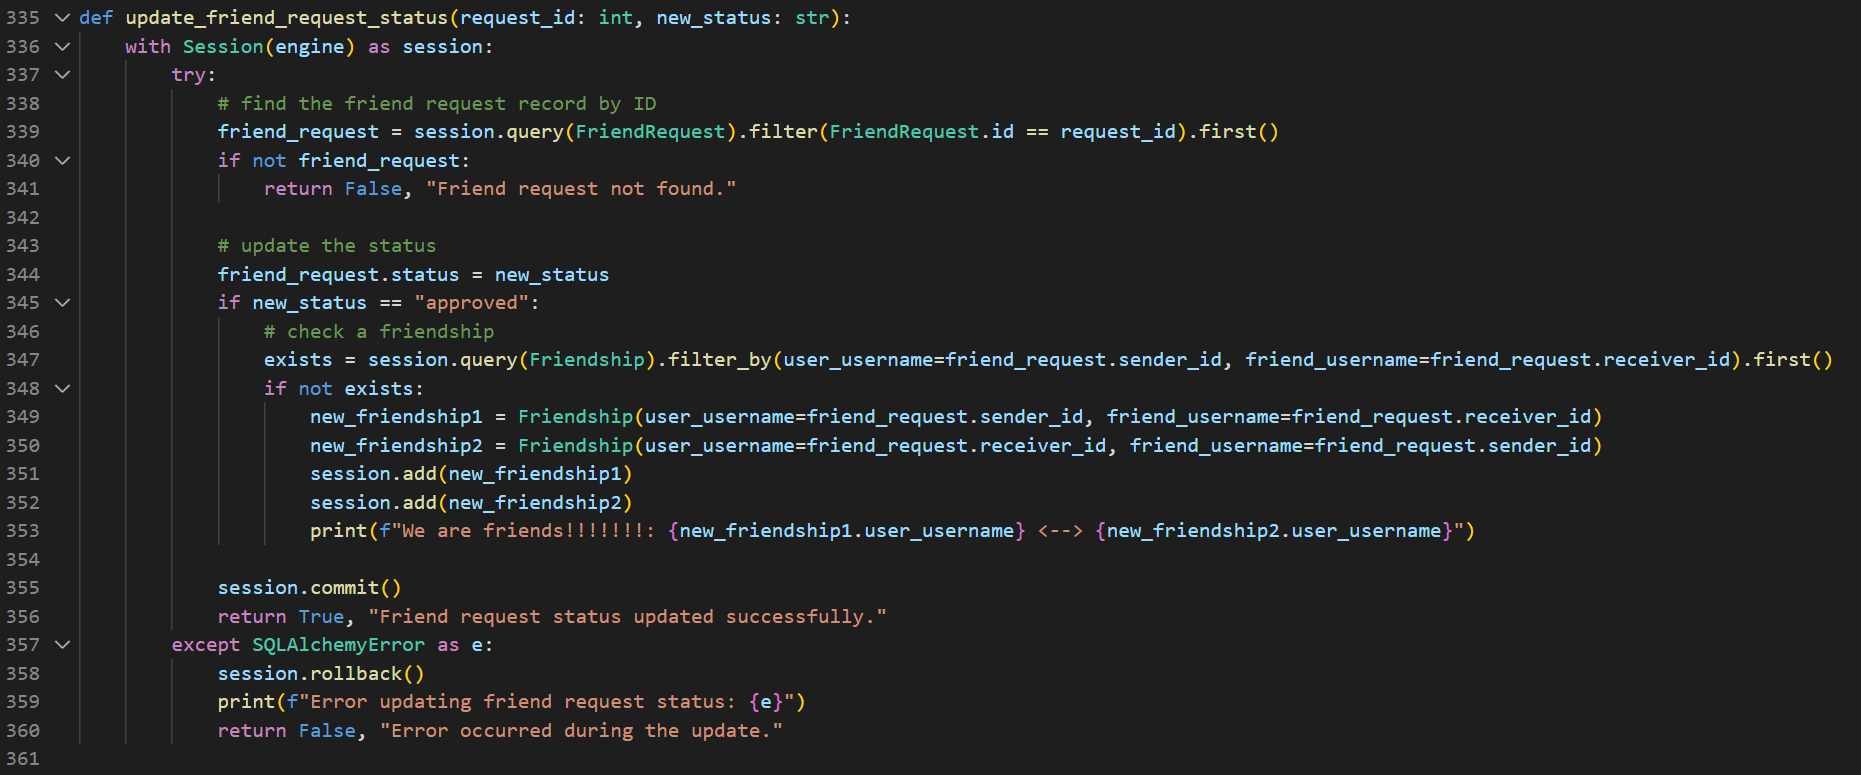
\includegraphics[width=0.8\textwidth]{zzrgraphs/db_update_request_status.png}
                \caption{db.py: update request status after user's operation}
                \label{updatestatus}
            \end{figure}

		\begin{figure}[H]
                \centering
                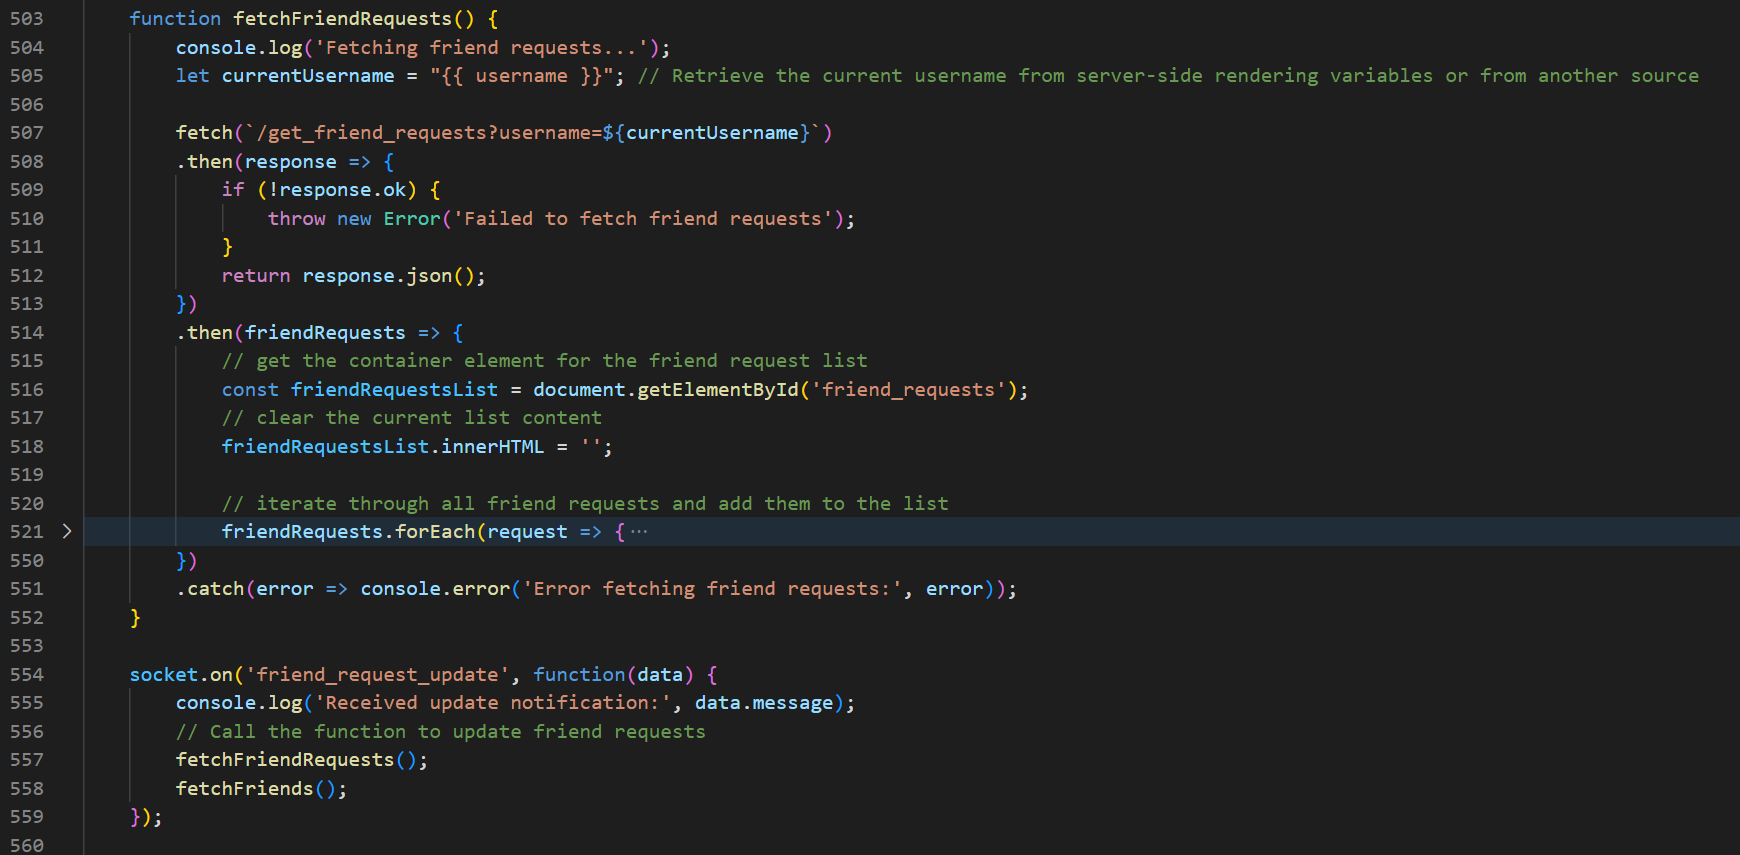
\includegraphics[width=0.8\textwidth]{zzrgraphs/home_fetchfriendrequests.png}
                \caption{home.jinja: fetch friendrequests and socket}
                \label{fetchrequests}
            \end{figure}
	
		\begin{figure}[H]
                \centering
                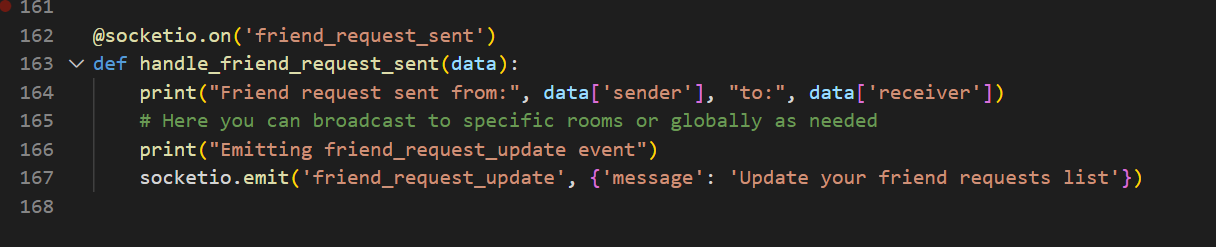
\includegraphics[width=0.8\textwidth]{zzrgraphs/socket_friend_request_sent.png}
                \caption{socket routes.py: listen to the frontend}
                \label{requestsocketio}
            \end{figure}

		\begin{figure}[H]
                \centering
                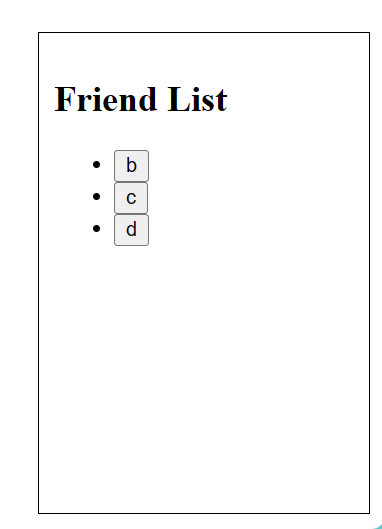
\includegraphics[width=0.2\textwidth]{zzrgraphs/friend_list.png}
                \caption{home page: friends are displayed as buttons}
                \label{friendlist}
            \end{figure}

		\begin{figure}[H]
                \centering
                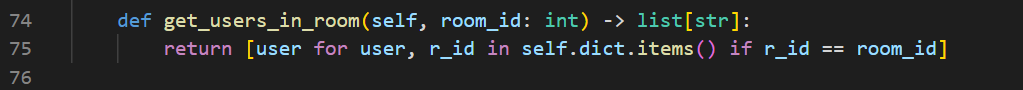
\includegraphics[width=0.8\textwidth]{zzrgraphs/models_get_users_in_room.png}
                \caption{models.py: check how many users are in the room}
                \label{getusersinroom}
            \end{figure}

		\begin{figure}[H]
                \centering
                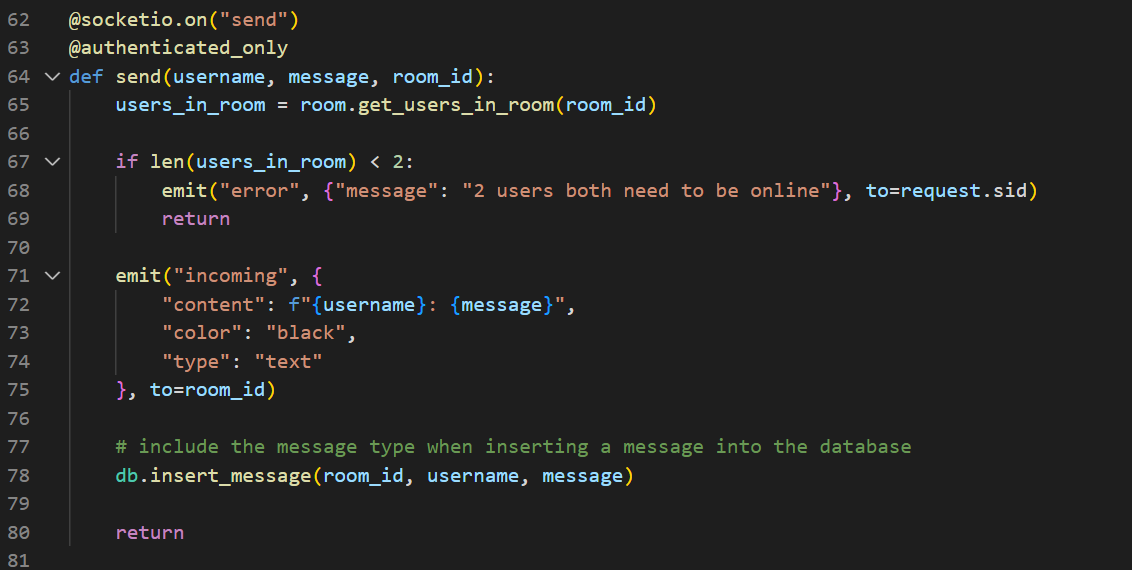
\includegraphics[width=0.8\textwidth]{zzrgraphs/socket_send.png}
                \caption{socket routes.py: check whether both users are online before sending message}
                \label{send}
            \end{figure}

            \begin{figure}[H]
                \centering
                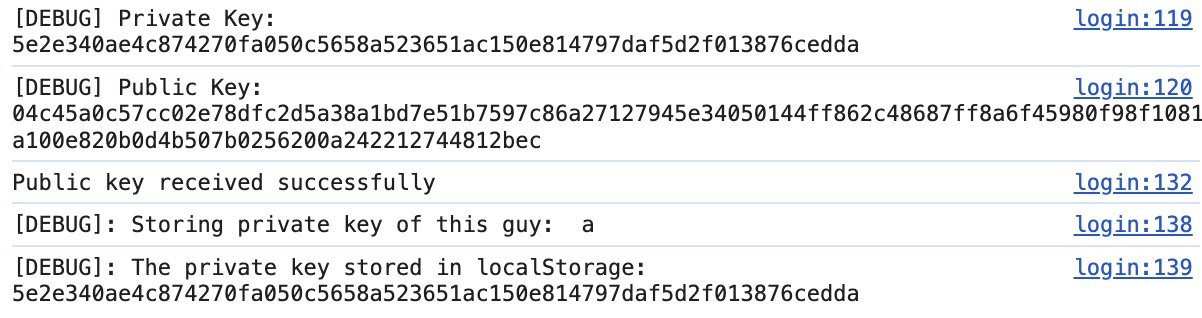
\includegraphics[width=0.8\textwidth]{graphs/show_keys.jpg}
                \caption{Illustration of private and public keys}
                \label{show_keys}
            \end{figure}

            \begin{figure}[H]
                \centering{}
                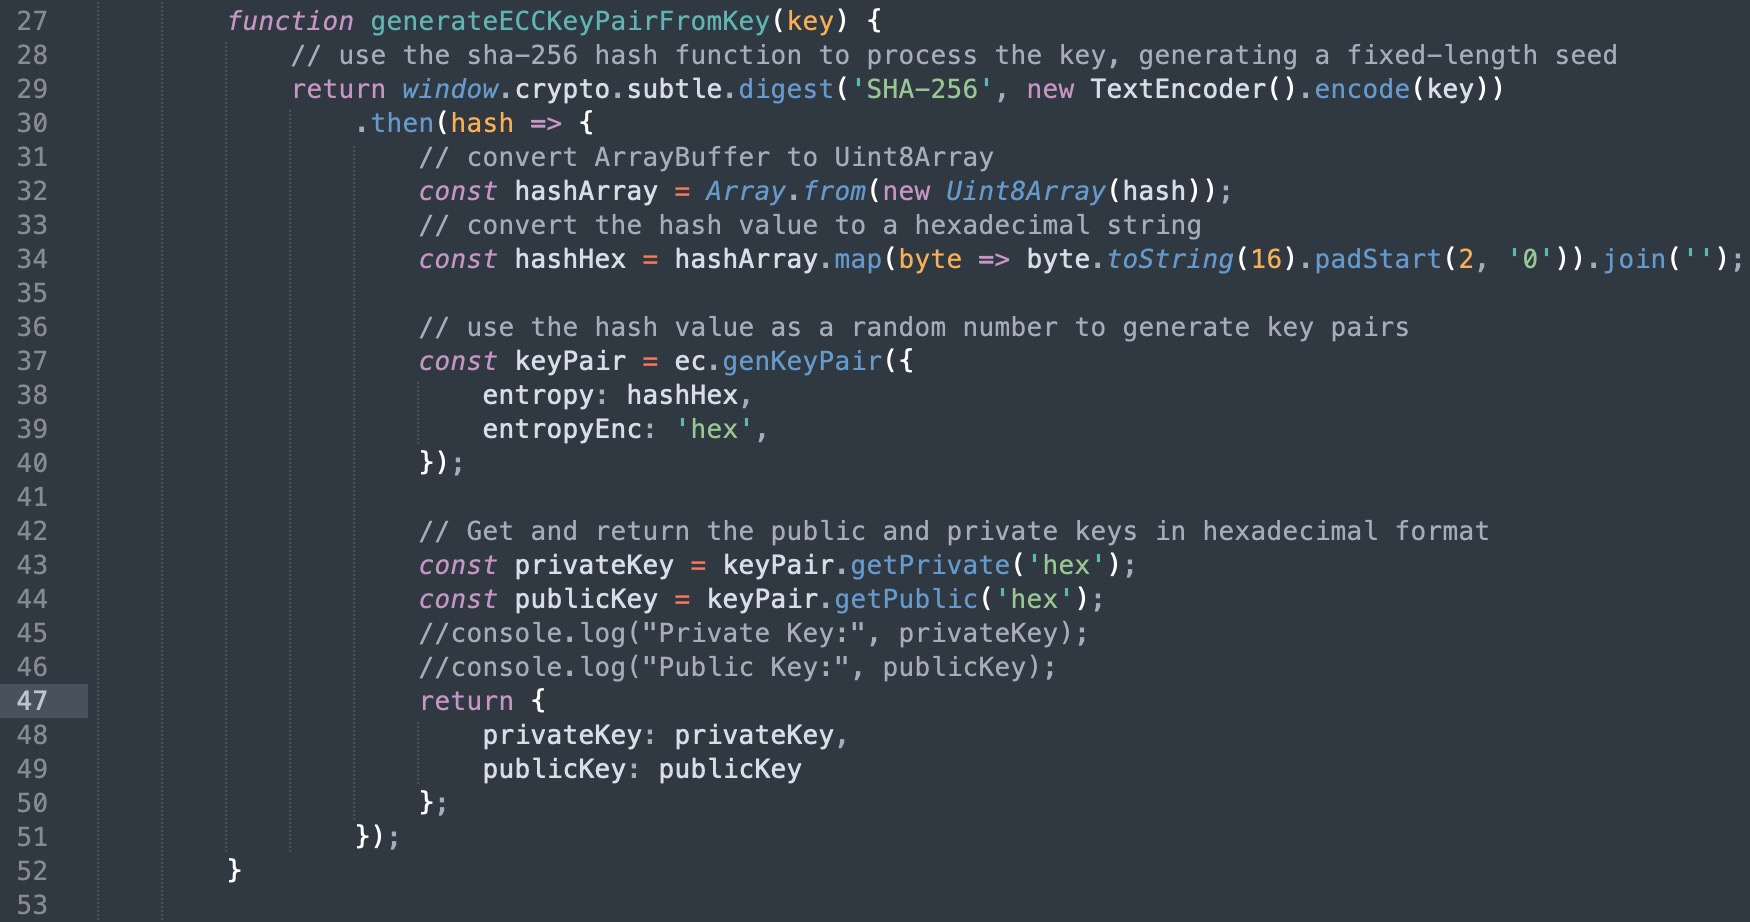
\includegraphics[width=0.8\textwidth]{graphs/generate_key_pairs.jpg}
                \caption{login.jinja \textit{line 16-54} and same function in signup.jinja \textit{line 27 - 65}}
                \label{generate_key_pairs}
            \end{figure}

            \begin{figure}[H]
                \centering{}
                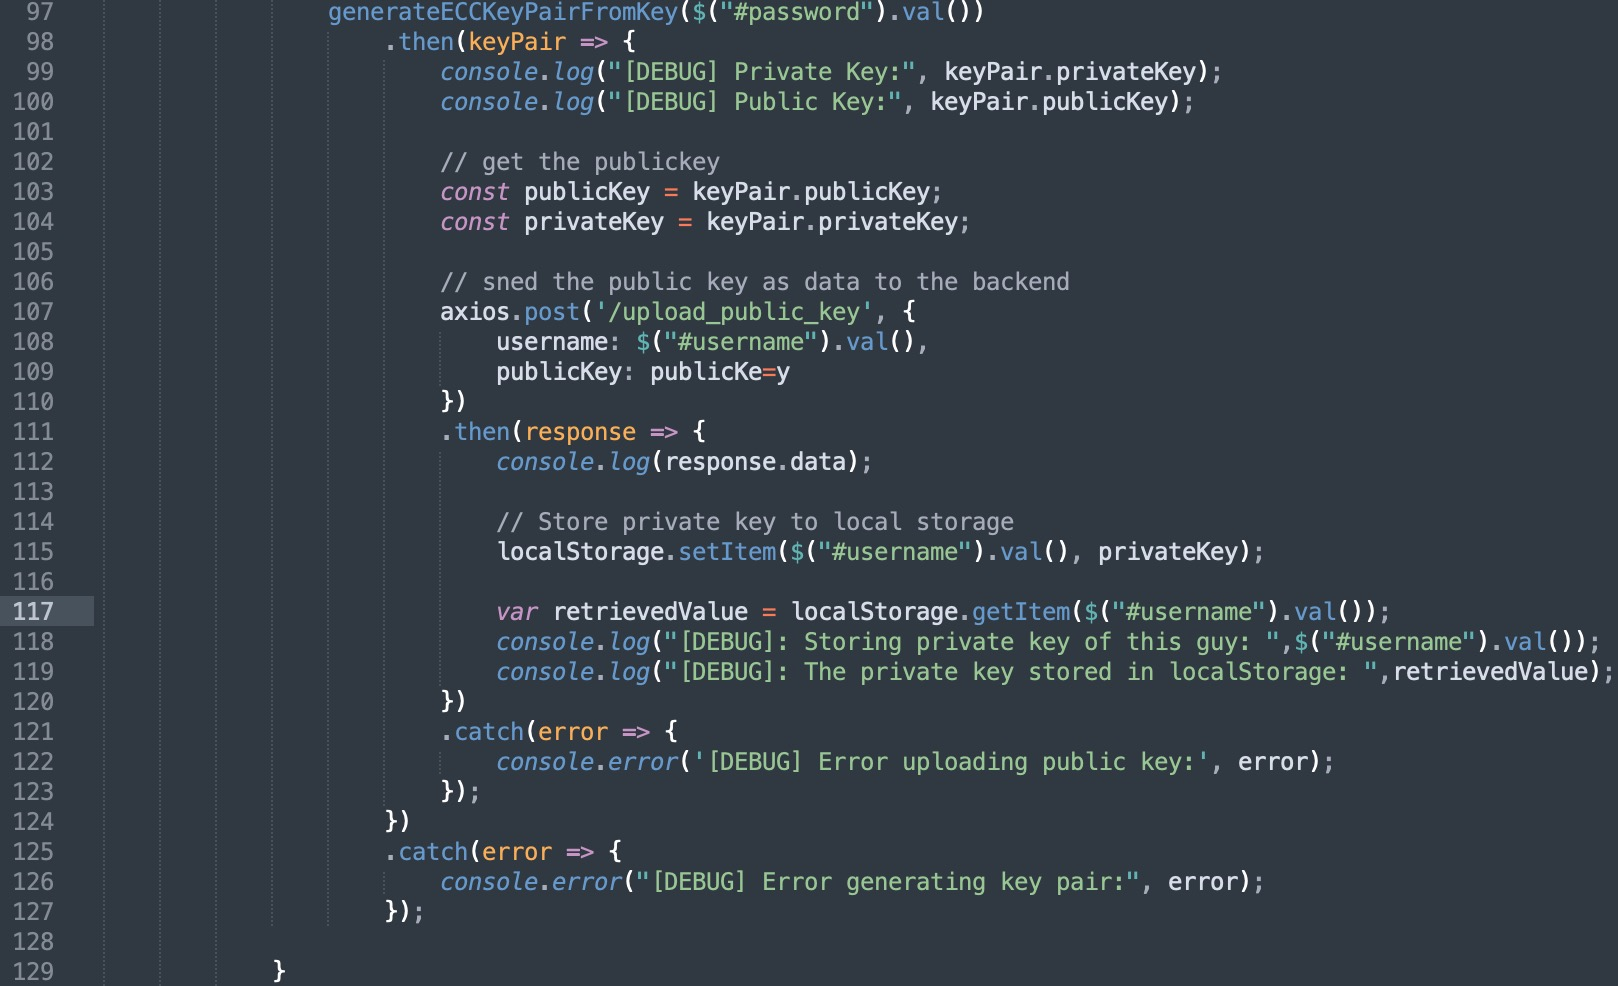
\includegraphics[width=0.7\textwidth]{graphs/store_key_pairs.jpg}
                \caption{login.jinja \textit{line 95-129} and same process in signup.jinja \textit{line 84 - 118}}
                \label{store_key_pairs}
            \end{figure}

            \begin{figure}[H]
                \centering
                \begin{subfigure}[b]{0.45\textwidth}
                    \centering
                    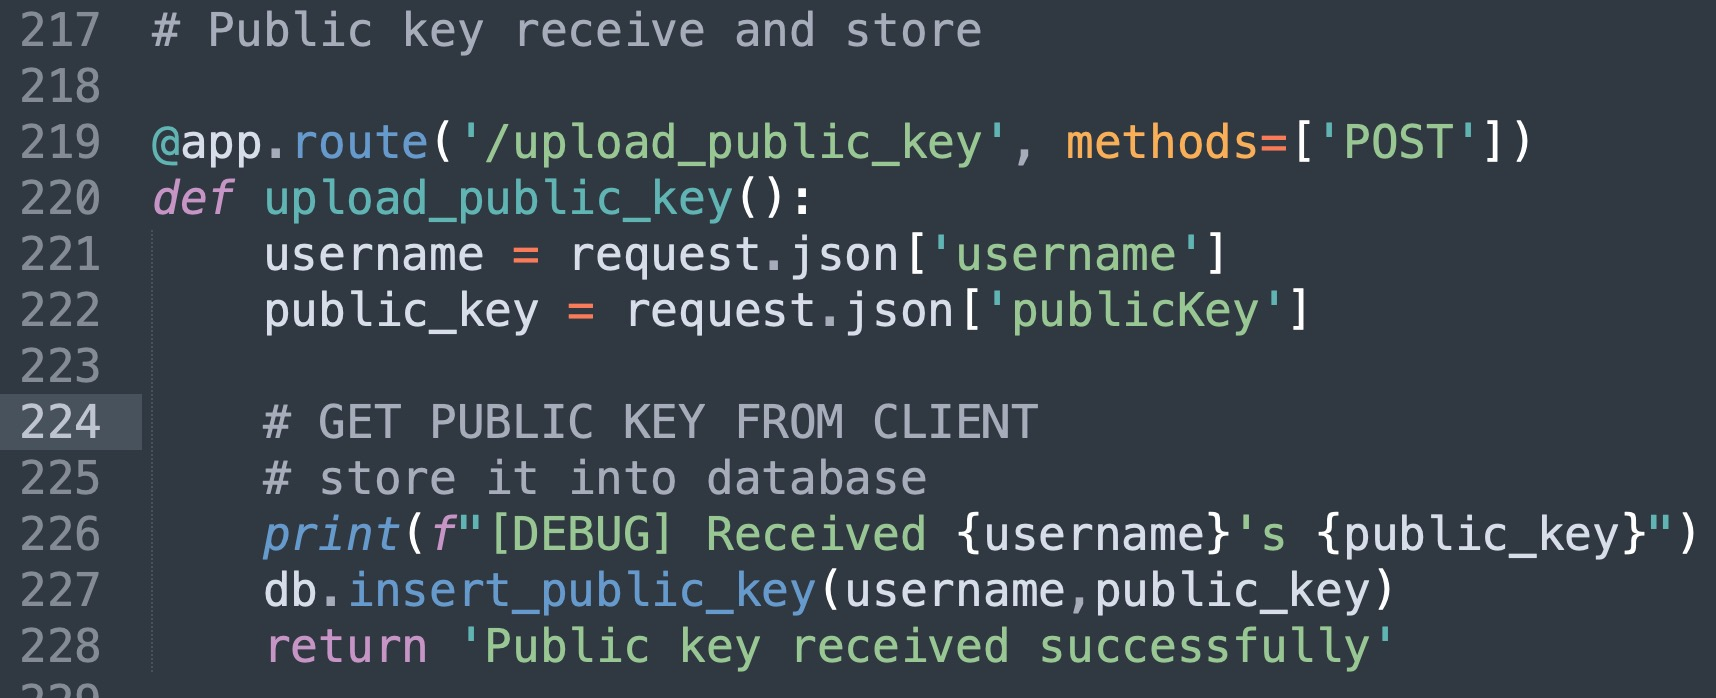
\includegraphics[width=\textwidth]{graphs/upload_public_key.jpg}
                    \caption{upload\_public\_key}
                \end{subfigure}
                \hfill 
                \begin{subfigure}[b]{0.45\textwidth}
                    \centering
                    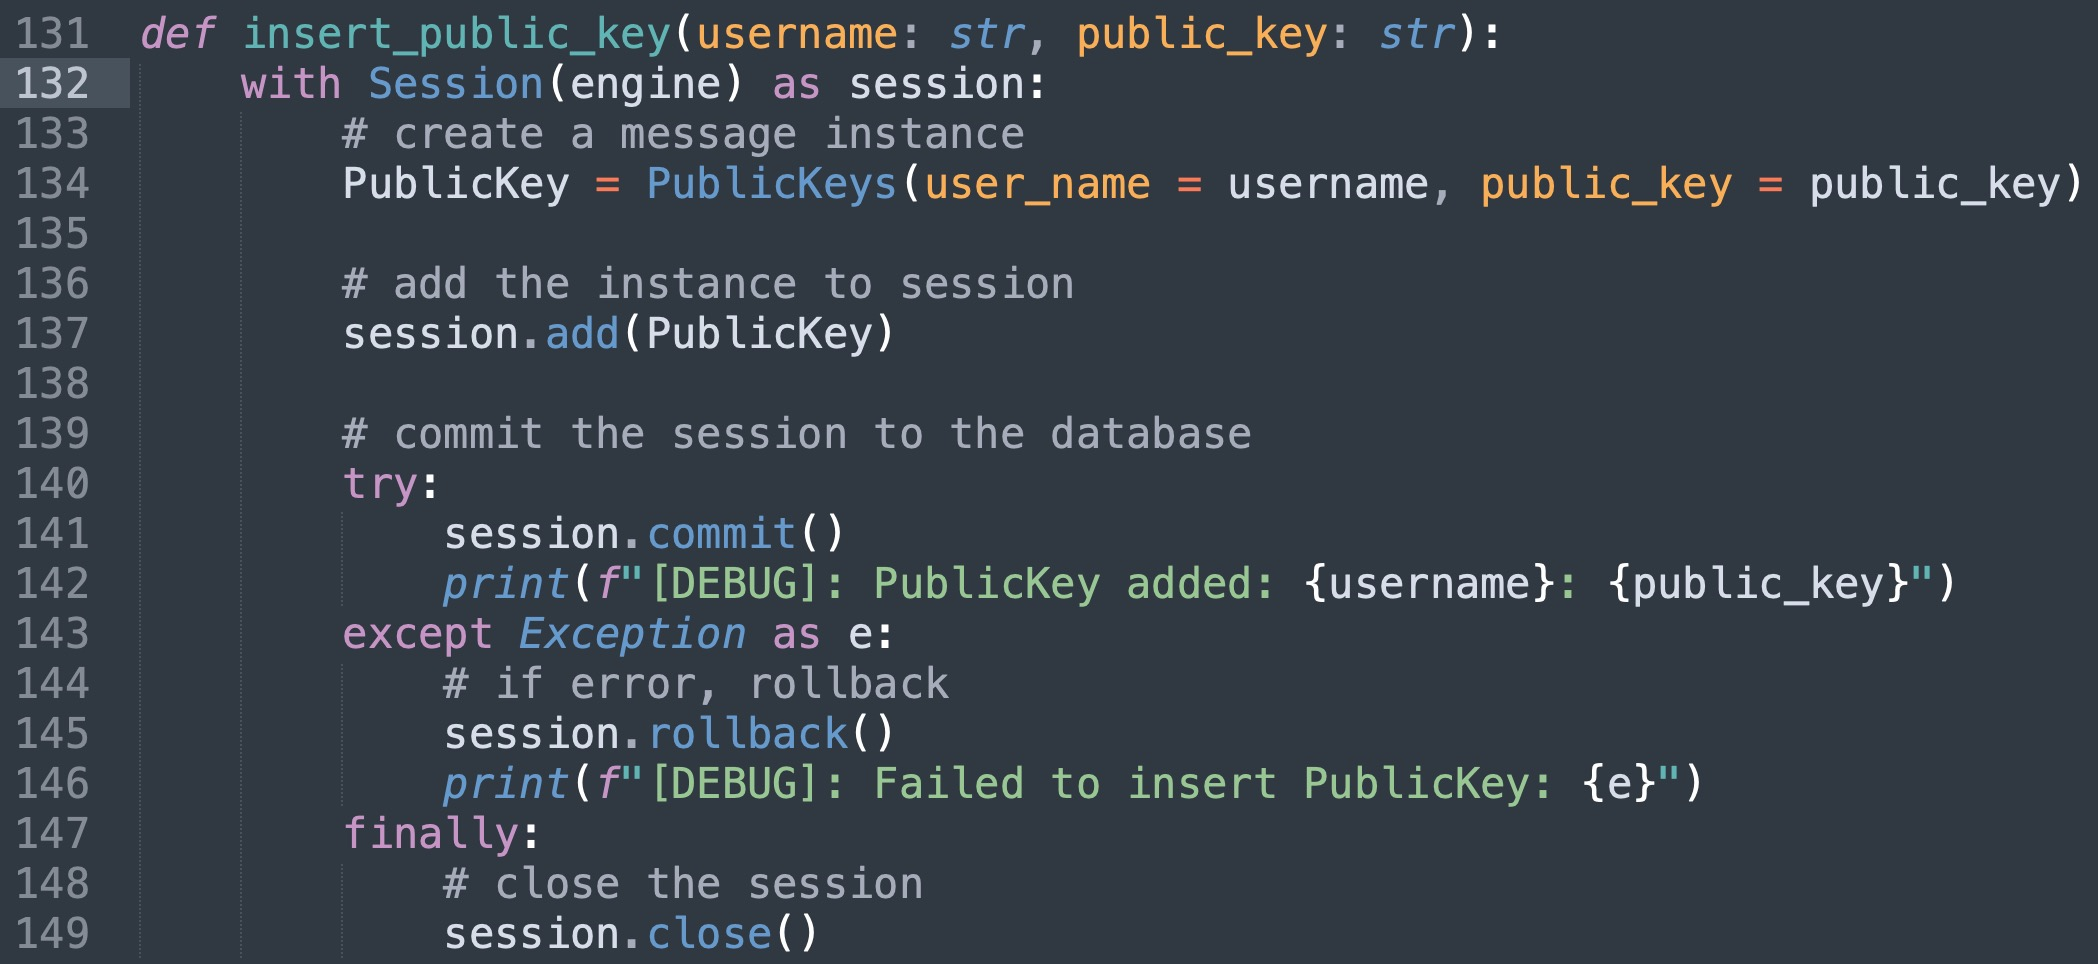
\includegraphics[width=\textwidth]{graphs/insert_public_key.jpg}
                    \caption{insert\_public\_key}
                \end{subfigure}
                \caption{Upload and Store public key}
                \label{Upload and Store public key}
            \end{figure}

            \begin{figure}[H]
                \centering
                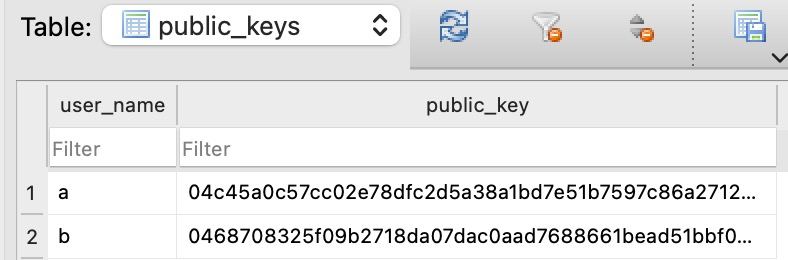
\includegraphics[width=0.8\textwidth]{graphs/db_public_key.jpg}
                \caption{main.db Table: public\_keys}
                \label{db public_key}
            \end{figure}

            \begin{figure}[H]
                \centering
                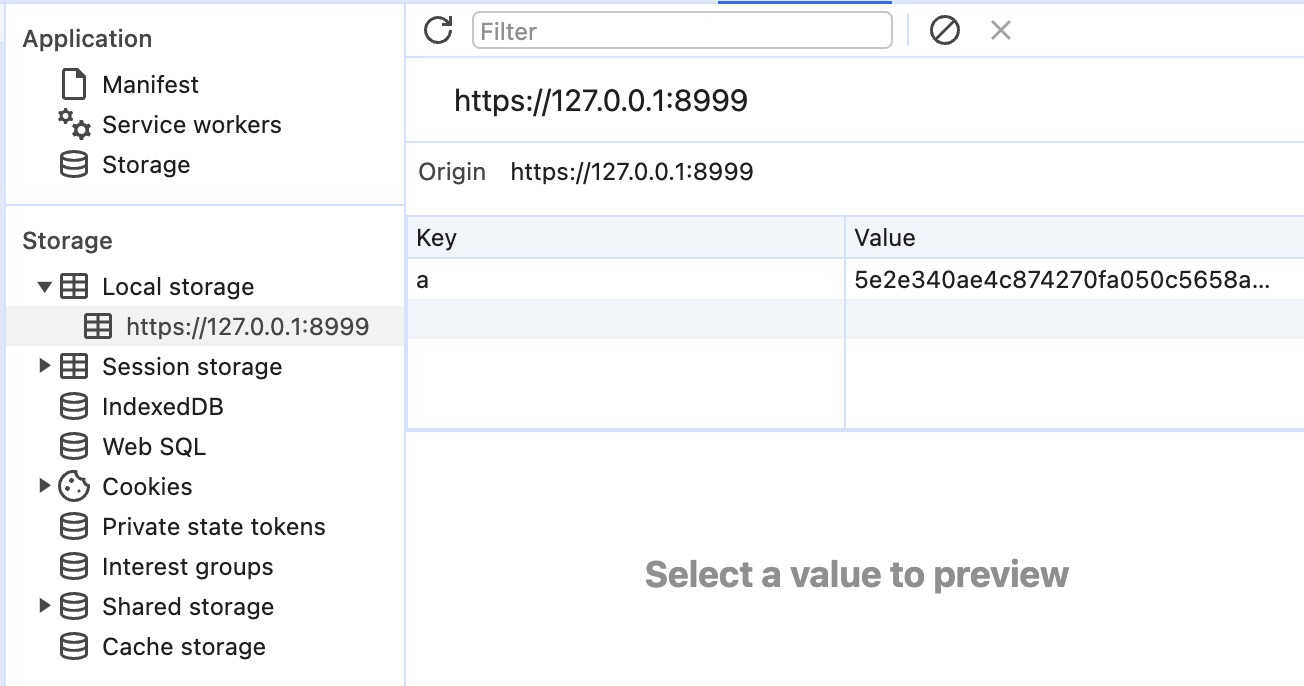
\includegraphics[width=0.8\textwidth]{graphs/local_storage.jpg}
                \caption{main.db Table: public\_keys}
                \label{local_storage}
            \end{figure}

            \item When a user enters a room shown in \ref{front join room}, the function \texttt{getPublicKey(receiver);} shown in \ref{get public key} called to request the public key of the conversing user from the server . The server retrieves the public key from the database and returns it shown in \ref{get and return public key}, storing it in a global variable in \texttt{home.jinja}. 

            When a user sends a message using the \texttt{send} function, they first generate a digital signature, as shown in Figure \ref{sign message}, using their own private key in local storage and the recipient's public key, previously obtained through \texttt{getPublicKey(receiver);} and stored in the global variable in \texttt{home.jinja}. This process utilizes Elliptic Curve Cryptography (ECC) to ensure the message's integrity and authentication. The digital signature is then incorporated into the message itself before it is sent.

            Following this, the function computes a shared key between two users using Elliptic Curve Cryptography (ECC) from hexadecimal representations of a private key and a public key, as shown in Figure \ref{compute shared key}. It converts the private key into a key pair object and the public key into a public key object. A shared key is then derived using these keys, serving as a secure basis for encrypted communication between the two users. Despite the involvement of individual private keys and the corresponding public key, both parties arrive at the same shared secret key. Thus, we successfully obtain a shared key that can be used for encrypting and decrypting messages, having exchanged only the public keys.


            \begin{figure}[H]
                \centering{}
                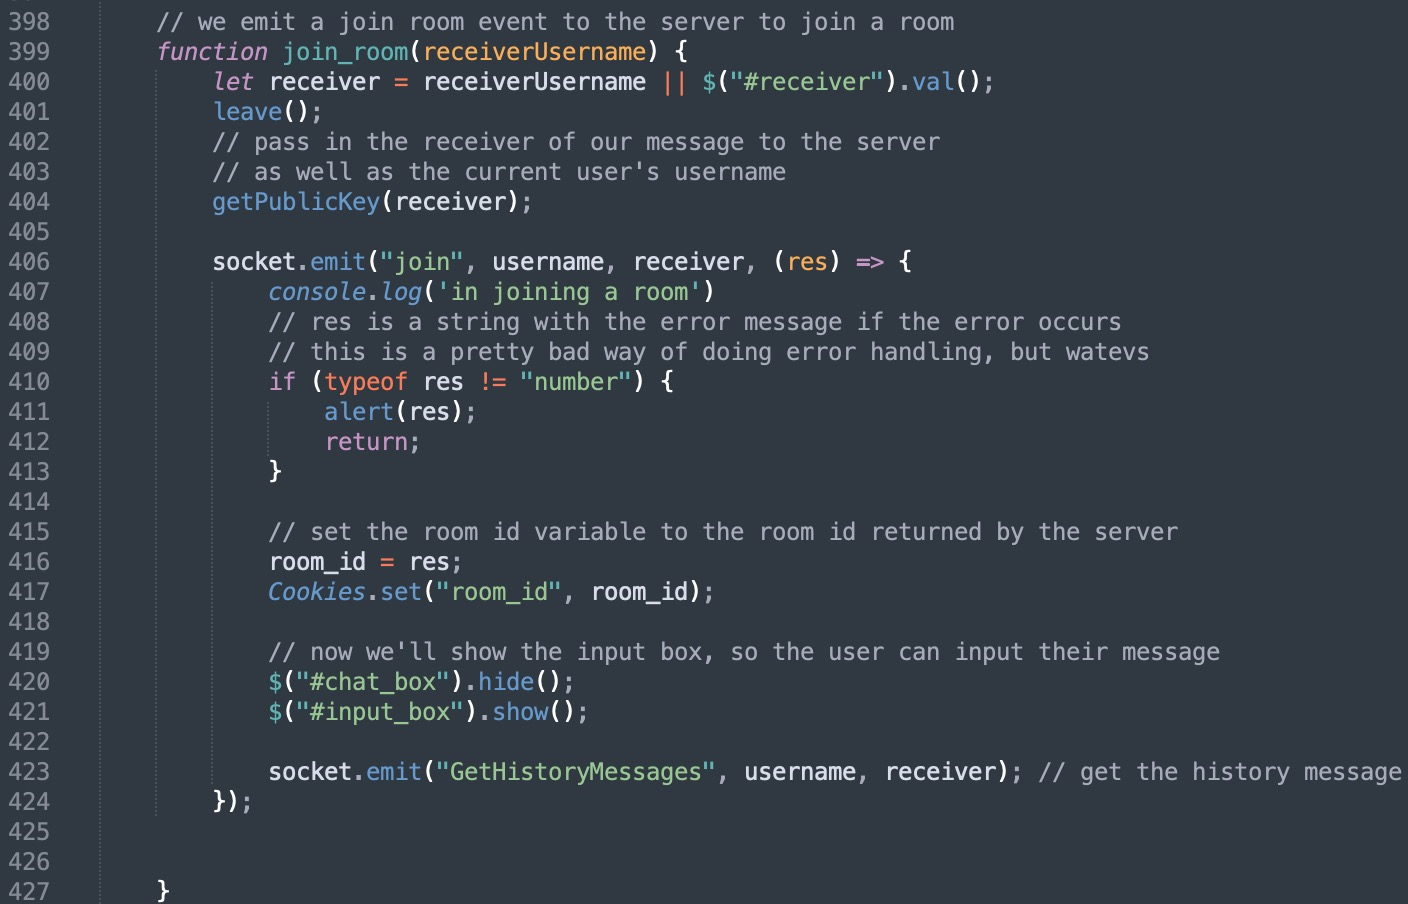
\includegraphics[width=0.8\textwidth]{graphs/front_join_room.jpg}
                \caption{home.jinja join\_room}
                \label{front join room}
            \end{figure}

            \begin{figure}[H]
                \centering
                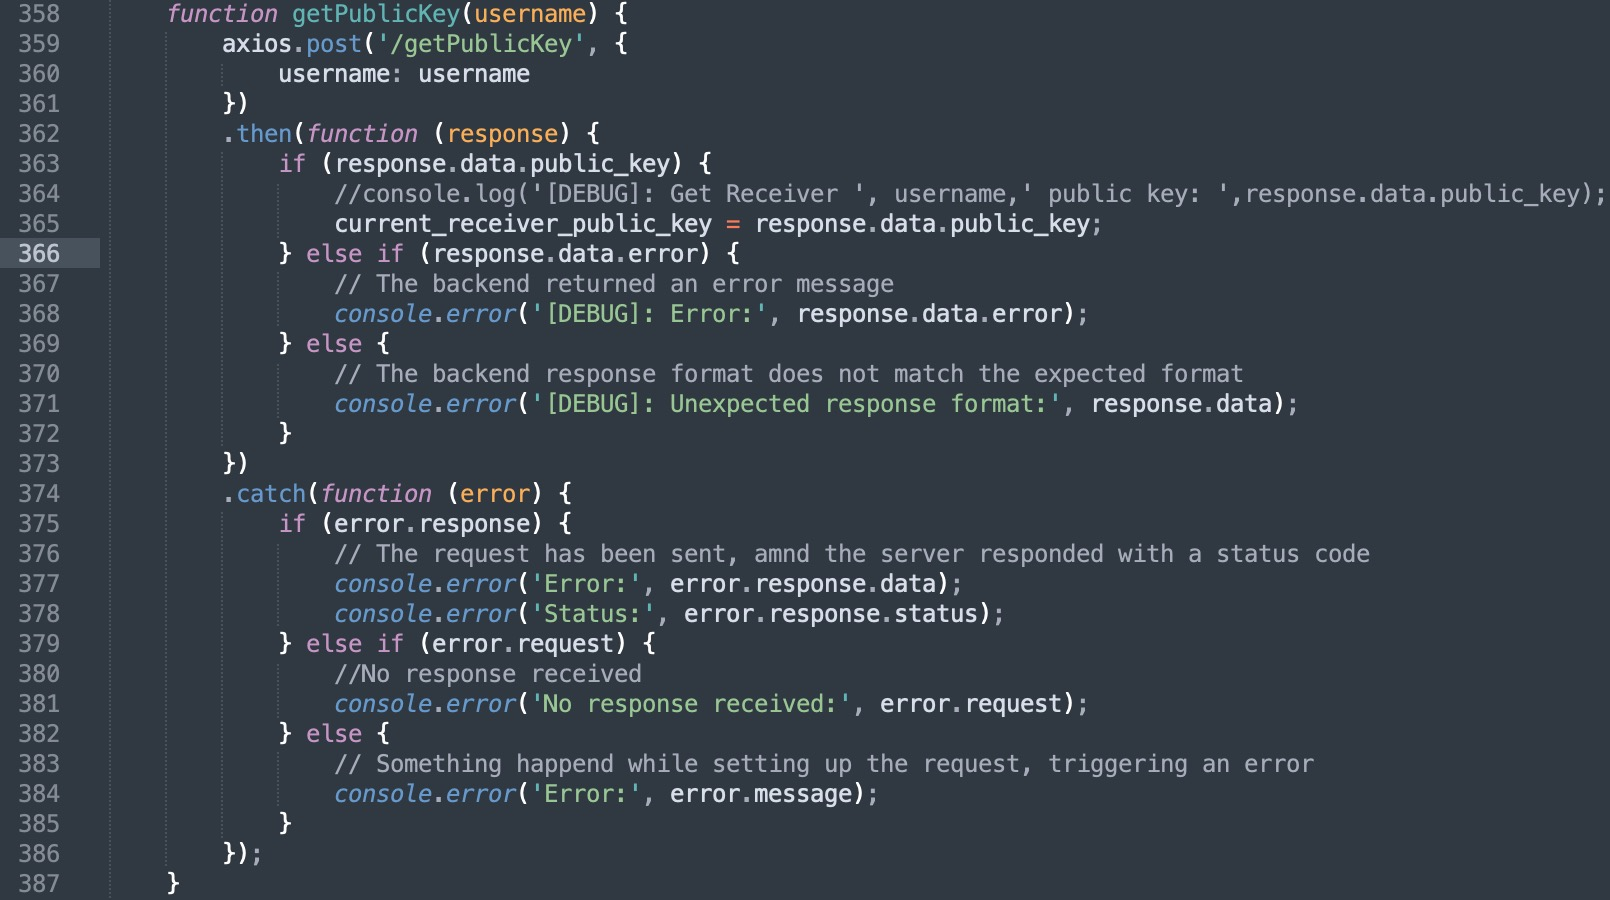
\includegraphics[width=0.8\textwidth]{graphs/front_get_public_key}
                \caption{home.jinja get\_public\_key}
                \label{get public key}
            \end{figure}


            \begin{figure}[H]
                \centering
                \begin{subfigure}[b]{0.47\textwidth}
                    \centering
                    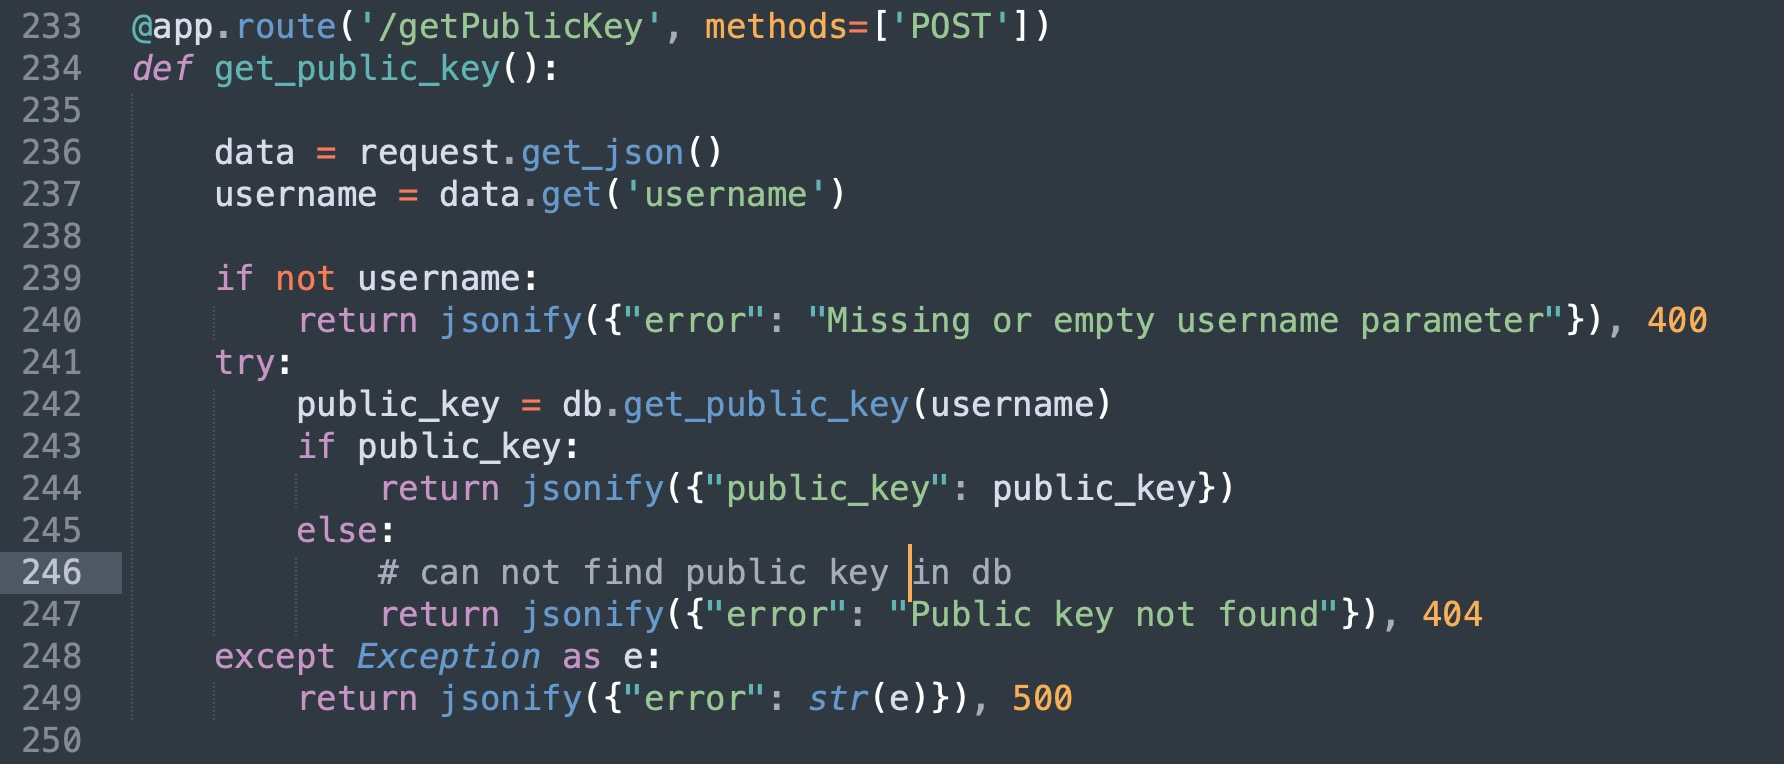
\includegraphics[width=\textwidth]{graphs/back_get_public_key.jpg}
                    \caption{app.py get\_public\_key \textit{line 230 - 246}}
                \end{subfigure}
                \hfill 
                \begin{subfigure}[b]{0.47\textwidth}
                    \centering
                    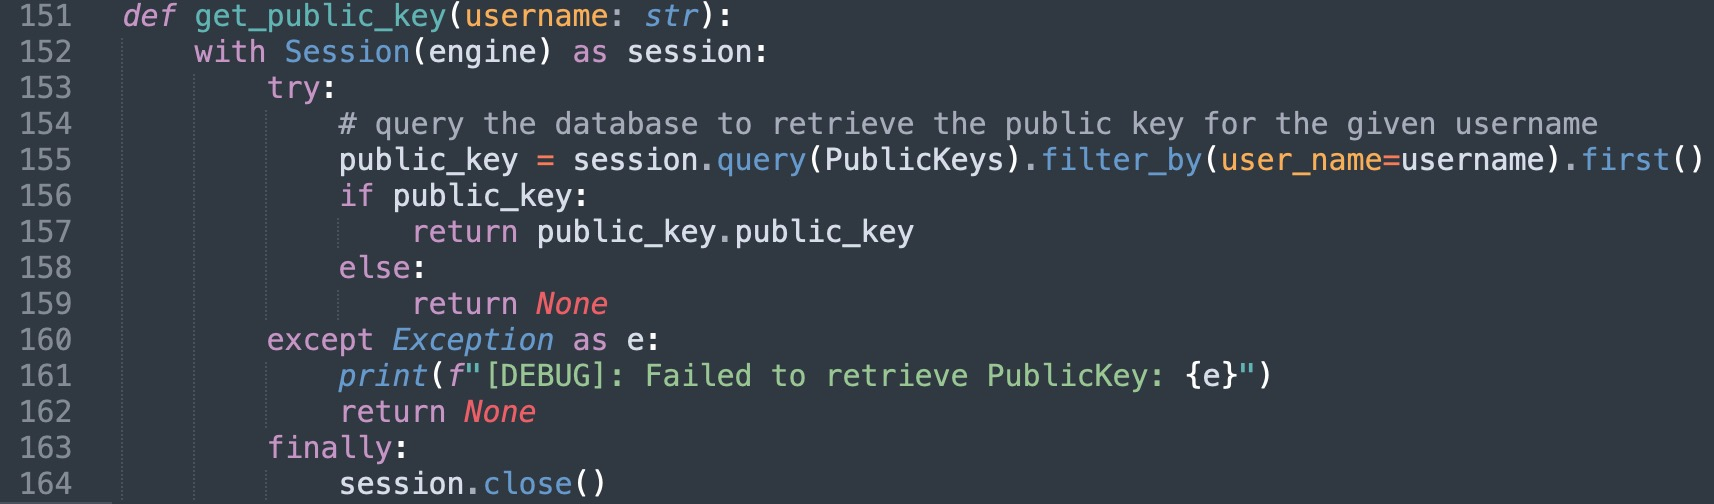
\includegraphics[width=\textwidth]{graphs/db_get_public_key.jpg}
                    \caption{db.py get\_public\_key \textit{line 151 - 164}}
                \end{subfigure}
                \caption{Get and return public key}
                \label{get and return public key}
            \end{figure}

            \begin{figure}[H]
                \centering
                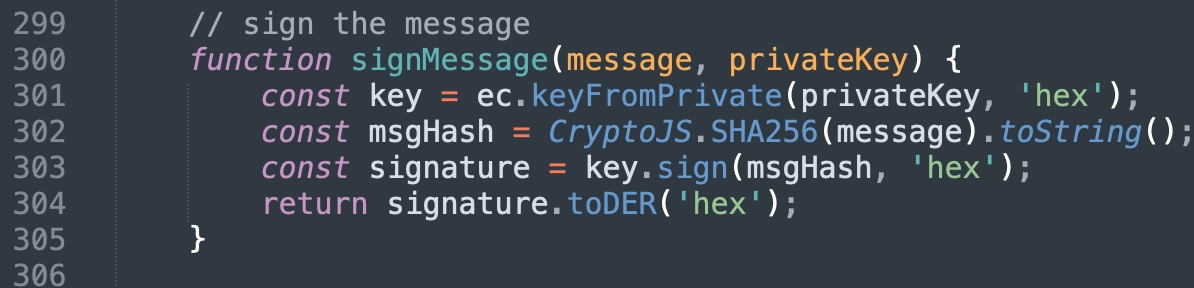
\includegraphics[width=0.8\textwidth]{graphs/sign_message.jpg}
                \caption{home.jinja signMessage \textit{line 299 - 305}}
                \label{sign message}
            \end{figure}

            \begin{figure}[H]
                \centering
                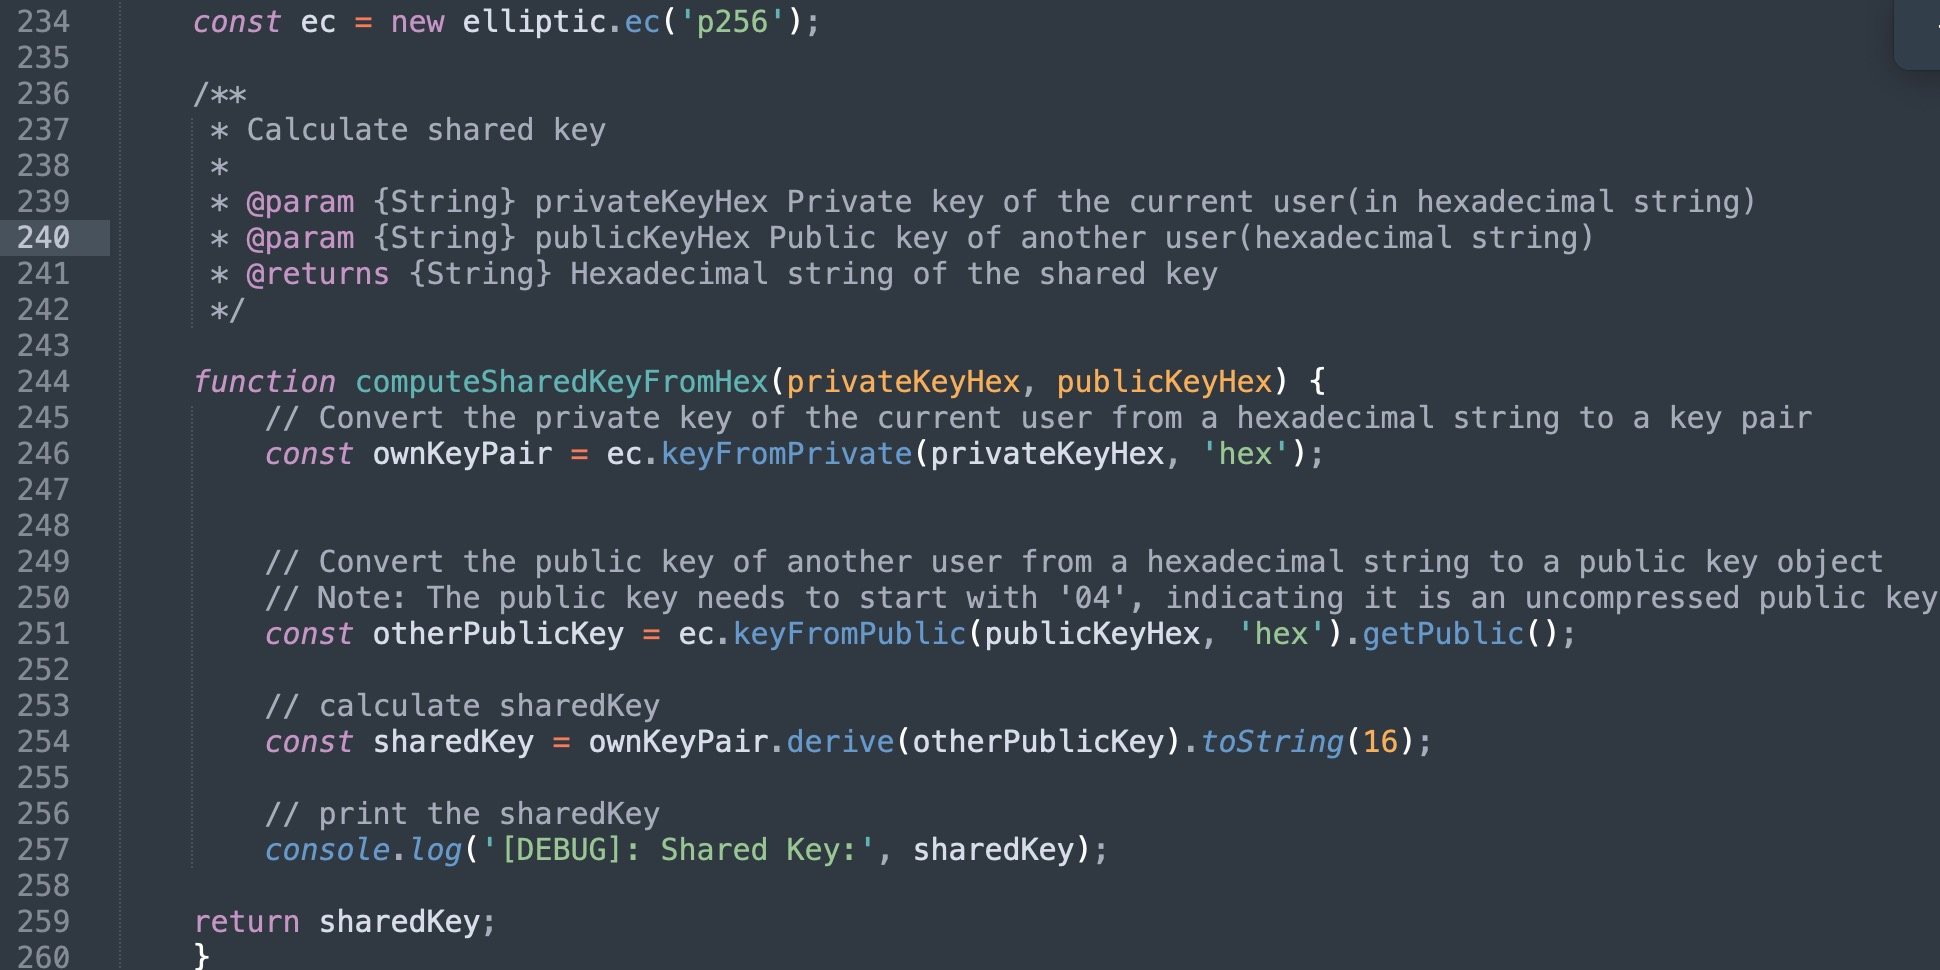
\includegraphics[width=0.8\textwidth]{graphs/compute_shared_key.jpg}
                \caption{home.jinja ComputeSharedKeyFromHex \textit{line 234 - 260}}
                \label{compute shared key}
            \end{figure}


            \item Subsequently, the \texttt{encryptMessage} function is called to encrypt the signed message using the AES algorithm through the CryptoJS library, as shown in \ref{encrypt message}. Initially, the shared key is converted from a hexadecimal string into the format required by the library. Then, the message is encrypted using a specified encryption mode and padding method. Finally, the encrypted, signed message is returned in string form and sent. The server only knows the public key and the encrypted message; thus, even if an attacker gains access to the server, they cannot decipher the message without knowing the user's private key.


            \begin{figure}[H]
                \centering
                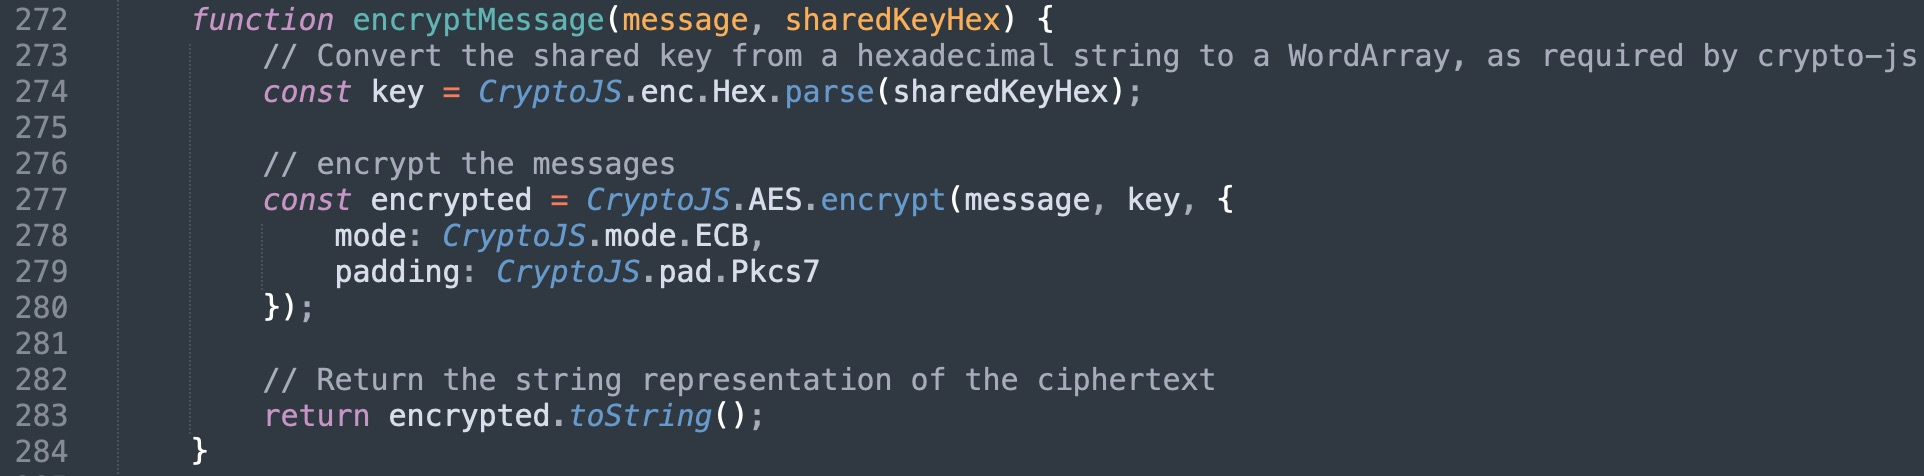
\includegraphics[width=0.8\textwidth]{graphs/encrypt_message.jpg}
                \caption{home.jinja encryptMessage \textit{line 260 - 272}}
                \label{encrypt message}
            \end{figure}

            \item When the recipient receives the encrypted message, the \texttt{incoming} event first calls the \texttt{processMessage} function, as shown in Figure \ref{processMessage}, to decrypt and verify the data. Similar to the previously mentioned process, a shared key is calculated using the sender's public key and the recipient's private key. The message is then decrypted using the \texttt{decryptMessage} function, as shown in Figure \ref{decryptMessage}. Following decryption, the sender's public key is used to verify the signature, as shown in Figure \ref{verify signature}. If all checks are successful, the message is displayed in the message box.


            \begin{figure}[H]
                \centering
                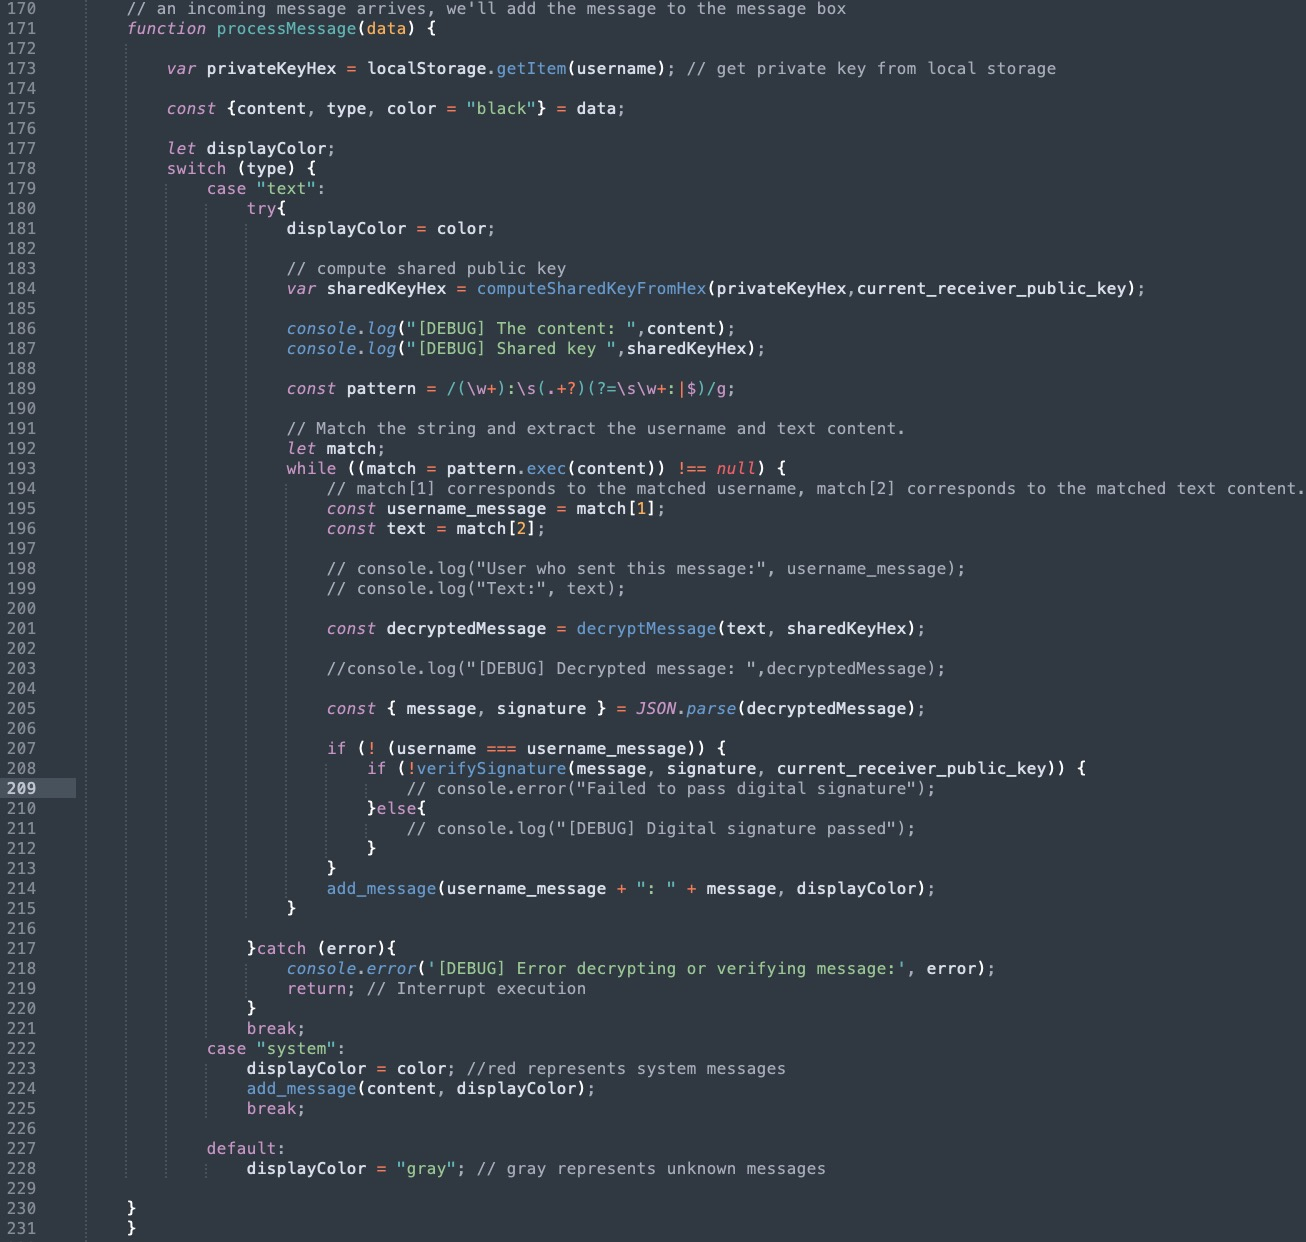
\includegraphics[width=0.8\textwidth]{graphs/processData.jpg}
                \caption{home.jinja processMessage \textit{line 260 - 272}}
                \label{processMessage}
            \end{figure}

            \begin{figure}[H]
                \centering
                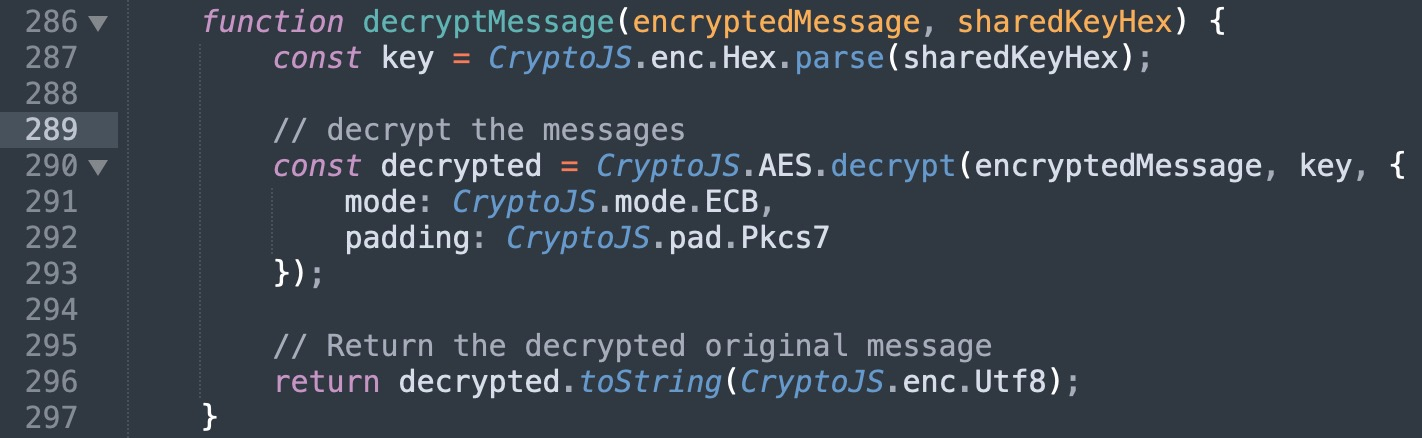
\includegraphics[width=0.8\textwidth]{graphs/decrypt_message.jpg}
                \caption{home.jinja decryptMessage \textit{line 260 - 272}}
                \label{decryptMessage}
            \end{figure}

            \begin{figure}[H]
                \centering
                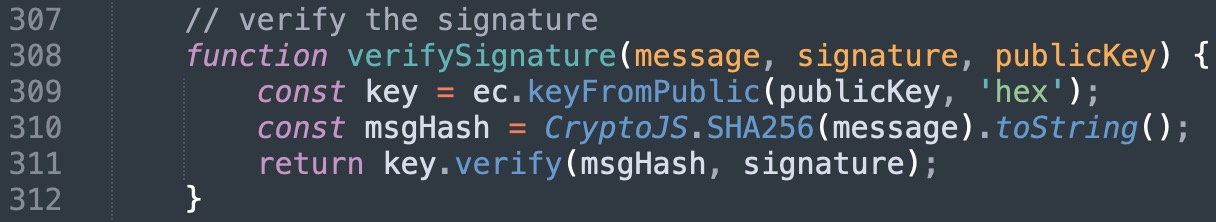
\includegraphics[width=0.8\textwidth]{graphs/verify_signature.jpg}
                \caption{home.jinja decryptMessage \textit{line 260 - 272}}
                \label{verify signature}
            \end{figure}

        \item The above process combines both symmetric and asymmetric encryption and utilizes digital signatures for message authentication. Through the ECC elliptic curve encryption algorithm, we enable two users to obtain the same shared key by only exchanging public keys. This shared key is then used to encrypt messages, with the server merely acting as an intermediary. Both encryption and decryption are completed on the client side.

        \end{enumerate}


    \subsection*{Part: Additional Criteria:}

        \subsubsection*{1} When signing up, after checking if the user has already signed up, the server will generate a random salt and hash the password with this salt. Finally, it stores the username, salt, and hashed password in the database.

        \begin{figure}[H]
            \centering
            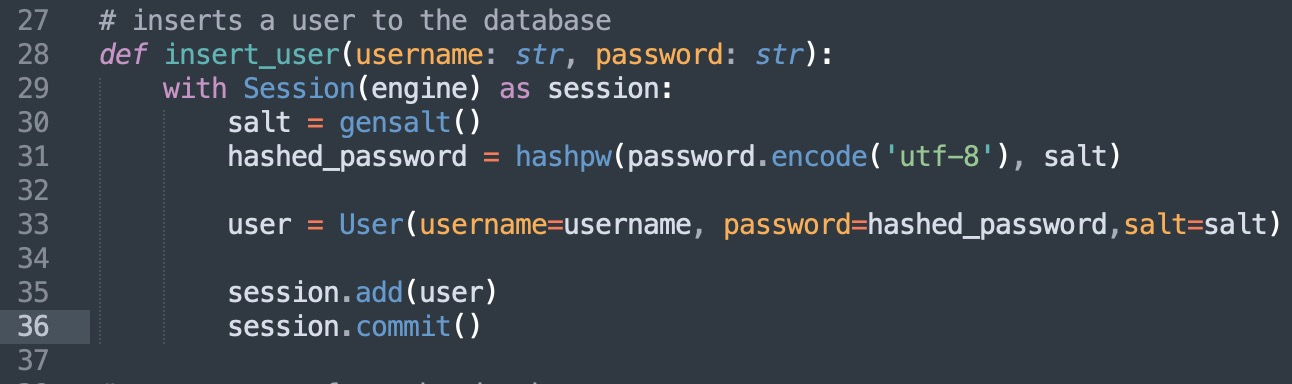
\includegraphics[width=0.8\textwidth]{graphs/insert_user.jpg}
            \caption{db.py insert\_user()}
        \end{figure}

        \begin{figure}[H]
            \centering
            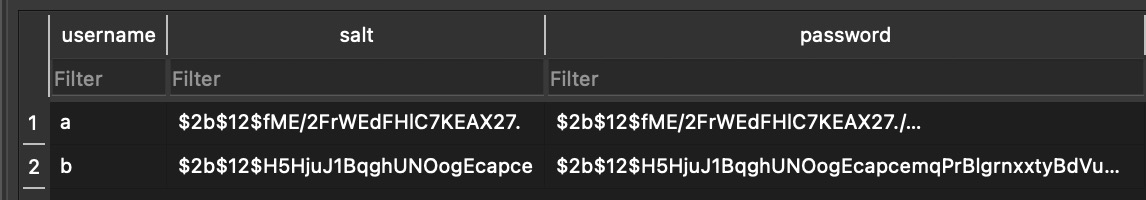
\includegraphics[width=0.8\textwidth]{graphs/hashed_passwd.jpg}
            \caption{main.db Table: user}
        \end{figure}

	\subsubsection*{2}Https:


In order to implement https to make our website more secure, we first create our own SSL certificate called myCA, then we use our own SSL certificate to create a CA-signed certificate called server for our messaging website. Then we tried adding our self-created certificate to the certificate manager to make the browser trust the HTTPS encryption of the localhost. However we encountered a SAN(Subject Alternative Name) issue. To solve this problem, we used a san.cnf file to re-edit the CA-signed certificate. After updating and reinstalling it into the certificate manager, we finally achieved the https encryption for localhost(shown in Figure \ref{certificates} Figure \ref{secureconnection}). We also insures that the user can only visit our website by https(shown in Figure \ref{httpsonly}), and there won't appear any browser warnings since the website is secure and trusted by the browser.


	\begin{figure}[H]
            \centering
            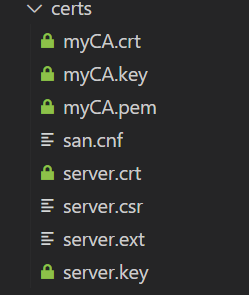
\includegraphics[width=0.8\textwidth]{zzrgraphs/certificates.png}
            \caption{all the certificates used in the project}
		\label{certificates}
        \end{figure}

	\begin{figure}[H]
            \centering
            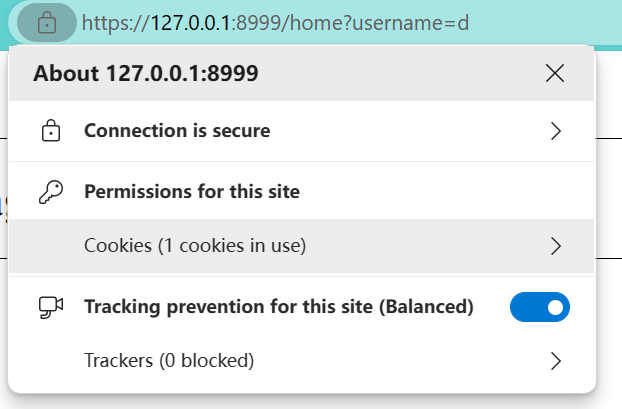
\includegraphics[width=0.8\textwidth]{zzrgraphs/connection_is_secure.png}
            \caption{the connection is secure by using https}
		\label{secureconnection}
        \end{figure}

	\begin{figure}[H]
            \centering
            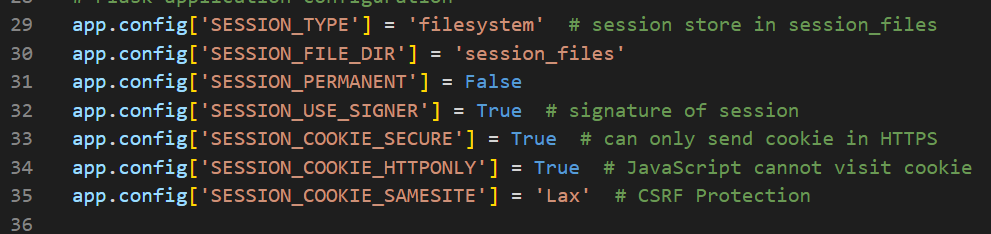
\includegraphics[width=0.8\textwidth]{zzrgraphs/cookie_secure_https_only.png}
            \caption{https only}
		\label{httpsonly}
        \end{figure}


\section{Contribution}

        \begin{verbatim}
            #include <iostream>

            int main() {
                std::cout << "Hello, World!" << std::endl;
                return 0;
            }
        \end{verbatim}

\end{document}